\section{Methodology}
\label{sec:method}

\subsection{Problem formulation}
A frequency-modulated continuous-wave (FMCW) mmWave radar outputs, at every
frame $t$, a small unordered set of detections
$\mathcal{F}_t=\{\mathbf{p}_{t,i}\}_{i=1}^{n_t}$ with
$\mathbf{p}=(x,y,z,v,\iota)$: the 3-D position, the radial (Doppler) velocity $v$
and the reflected intensity $\iota$. The count $n_t$ is small and varies
(median 21 on RadHAR and 6 on MiliPoint, Section~\ref{sec:data}). Given a
window $\mathcal{W}=(\mathcal{F}_{t_0},\dots,\mathcal{F}_{t_0+T-1})$ of $T$ frames
(2\,s), we learn $f_\theta:\mathcal{W}\mapsto\hat{y}\in\{1,\dots,K\}$ that
predicts the activity. $f_\theta$ must be invariant to the order of points within
a frame, robust to missing detections, and cheap enough to run on an edge device
at the radar frame rate. The radar never records an image of the person, so the
sensing is privacy-preserving by construction.

\subsection{Radar-specific pre-processing}
\label{sec:preproc}
Raw RadHAR windows contain three kinds of returns (Fig.~\ref{fig:preproc}):
antenna self-returns at $x\approx0$, static multipath and clutter several metres
behind the subject, and the person. We apply three steps.
\textbf{(i) ROI}: drop returns with $x<0.3$\,m (34.6\% of all points).
\textbf{(ii) Person centring}: the window centre $\mathbf{c}$ is the median
position of the \emph{moving} returns ($v\neq0$), because static clutter has
zero radial velocity; if a window has no moving return we fall back to the median of
all returns. Coordinates are expressed relative to $\mathbf{c}$, which removes
the subject's absolute position and distance from the radar.
\textbf{(iii) Spatial gating}: returns farther than $r_g=1.2$\,m (horizontally)
from $\mathbf{c}$ are discarded. This removes on average 50.1\% of the remaining
returns, almost all of them static clutter. Gating also removes a shortcut: the
same furniture appears in training and test recordings, so a model could use
the clutter to recognise the scene instead of the motion.
MiliPoint is already cropped to the subject and has no Doppler channel, so only
median centring is applied. Its axes are remapped to the RadHAR convention ($x$
forward, $y$ lateral, $z$ up) so that both datasets share one coordinate frame.

\begin{figure}[t]
\centering
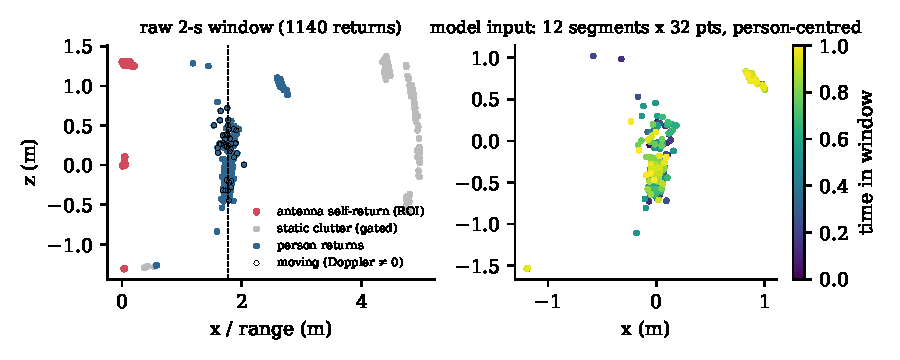
\includegraphics[width=\columnwidth]{../figures/preproc_before_after.pdf}
\caption{A raw 2-s RadHAR window (left): antenna self-returns (red), static
clutter removed by gating (grey), person returns (blue) and moving returns
(circled). Right: the resulting person-centred model input, coloured by time.}
\label{fig:preproc}
\end{figure}

\textbf{Temporal segmentation and sampling.} A window is split into $G=12$
equal segments (5 frames on RadHAR at 30\,Hz and 4 frames on MiliPoint at 24\,Hz).
From each segment we sample $P=32$ returns, with replacement when fewer exist.
This gives a fixed tensor $\mathbf{X}\in\mathbb{R}^{G\times P\times C}$ with
$C=6$ features: centred $x,y,z$; $v$; $\iota$ standardised with training
statistics; and the normalised time inside the window. A mask
$\mathbf{M}\in\{0,1\}^{G\times P}$ marks empty segments. Accumulating a few
frames per segment counters the extreme sparsity of single frames while keeping
temporal order across segments.

\textbf{Augmentation (training only).} Random rotation about the vertical axis
($\pm15^\circ$), isotropic scaling ($[0.9,1.1]$), Gaussian jitter
($\sigma=1$\,cm) and fresh random point sampling at every epoch.

\begin{figure*}[t]
\centering
\begin{tikzpicture}[
  font=\scriptsize, >=latex,
  box/.style={draw, rounded corners=2pt, align=center, minimum height=7mm, inner sep=2pt},
  frozen/.style={box, fill=blue!8},
  train/.style={box, fill=orange!15},
  mot/.style={box, fill=green!12},
  ]
\node[box, fill=gray!10, minimum width=17mm] (in) {radar window\\$60$ frames, $2$\,s\\$(x,y,z,v,\iota)$};
\node[box, right=4mm of in, minimum width=19mm, fill=gray!10] (pre) {ROI + moving-\\point centring +\\$1.2$\,m gating};
\node[box, right=4mm of pre, minimum width=16mm, fill=gray!10] (seg) {$G{=}12$ segments\\$\times P{=}32$ pts\\$\mathbf{X}\in\mathbb{R}^{12\times32\times6}$};
\node[train, right=6mm of seg, minimum width=26mm] (tok) {\textbf{Segment tokenizer}\\shared point MLP $6{\to}64$\\point self-attn. + rel.-pos. bias\\attentive \& max pooling};
\node[mot, below=4mm of tok, minimum width=26mm] (md) {\textbf{Motion descriptor}\\centroid, $\Delta$centroid,\\$\overline{|v|}$, $\log n$ $\to$ MLP};
\node[circle, draw, right=4mm of tok, inner sep=1pt] (plus) {$+$};
\node[train, right=4mm of plus, minimum width=24mm] (tem) {\textbf{Temporal encoder}\\$[\mathrm{CLS}]$ + 12 tokens\\$2\times$ Transformer block\\($d{=}64$, 4 heads)};
\node[box, right=4mm of tem, minimum width=12mm, fill=red!10] (out) {LN +\\linear\\$\hat{y}$};
\draw[->] (in) -- (pre); \draw[->] (pre) -- (seg); \draw[->] (seg) -- (tok);
\draw[->] (seg.south) |- (md.west); \draw[->] (tok) -- (plus); \draw[->] (md.east) -| (plus.south);
\draw[->] (plus) -- (tem); \draw[->] (tem) -- (out);
\node[box, dashed, below=4mm of tem, minimum width=24mm, fill=yellow!10] (teach) {STPT-Large teacher\\($d{=}128$, 4 blocks)};
\draw[->, dashed] (teach.east) -| node[pos=0.75, right, align=left]{KD:\\$\mathrm{KL}(p_T^{\tau}\Vert p_S^{\tau})$} (out.south);
\end{tikzpicture}
\caption{STPT-Lite. Points are attended to only \emph{within} a short temporal
segment (cost $O(GP^2)$), each segment is compressed into one token enriched
with an explicit radar motion descriptor, and a small Transformer attends
\emph{across} the $G$ segment tokens ($O(G^2)$). No farthest-point sampling or
$k$-NN search is needed. A larger STPT teacher is distilled into the student,
whose weights are finally quantised to INT8.}
\label{fig:arch}
\end{figure*}

\subsection{STPT-Lite: a factorised spatio-temporal point transformer}
Generic point-cloud backbones (PointNet++, DGCNN, Point Transformer) treat the
accumulated window as one static set. They spend most of their computation on
farthest-point sampling and $k$-NN neighbourhoods over the whole set, and they
encode time only as one more coordinate. Radar HAR has the opposite structure:
very few points per instant, but strong regularity over time. STPT-Lite
(Fig.~\ref{fig:arch}) therefore factorises attention into a spatial part and a
temporal part.

\textbf{Segment tokenizer.} A shared MLP embeds every point,
$\mathbf{h}=\phi(\mathbf{x})\in\mathbb{R}^{d}$ ($d=64$). One pre-norm
multi-head self-attention block then runs over the $P$ points of each segment,
with a learned relative-position bias computed from pairwise 3-D offsets:
\begin{equation}
\mathbf{A}^{(h)}_{ij}=\operatorname{softmax}_j\!\Big(\tfrac{\mathbf{q}_i^{(h)}\cdot\mathbf{k}_j^{(h)}}{\sqrt{d/H}}+\beta^{(h)}(\mathbf{x}_i^{xyz}-\mathbf{x}_j^{xyz})+\log m_j\Big),
\end{equation}
where $\beta$ is a two-layer MLP $\mathbb{R}^3\!\to\!\mathbb{R}^{H}$ and $m_j$
is the mask. The block is followed by a feed-forward layer. The segment token
concatenates attentive pooling,
$\mathbf{a}=\sum_i\operatorname{softmax}_i(\mathbf{w}^\top\mathbf{h}_i)\mathbf{h}_i$,
with max pooling, and projects the result back to $d$ dimensions. Because $P=32$,
full attention inside a segment costs only $G\cdot P^2=12{,}288$ pairs, against
$(GP)^2\approx1.5\times10^5$ for joint attention over the window.

\textbf{Motion descriptor.} Radar measures motion directly, so we give it to the
model explicitly. For each segment $g$ we compute
$\mathbf{u}_g=[\bar{\mathbf{x}}_g,\;\bar{\mathbf{x}}_g-\bar{\mathbf{x}}_{g-1},\;\overline{|v|}_g,\;\log(1+n_g)]\in\mathbb{R}^8$,
i.e.\ the segment centroid, its displacement since the previous segment, the
mean Doppler magnitude and the log point count. An MLP embeds $\mathbf{u}_g$,
and the result is added to the segment token.

\textbf{Temporal encoder.} A learnable [CLS] token and positional embeddings are
prepended to the $G$ tokens, which pass through $L=2$ pre-norm Transformer blocks
\cite{vaswani2017attention} ($H=4$ heads, FFN width $2d$). Empty segments are
masked. The final [CLS] state is layer-normalised and classified. The whole model
has 117.5\,K parameters and needs 36.6\,MFLOPs per 2-s window.

\subsection{Knowledge distillation and quantisation}
A wider teacher (STPT-Large: $d=128$, 4 temporal blocks, 8 heads, 725\,K
parameters) is trained first. The student minimises
\begin{equation}
\mathcal{L}=(1-\alpha)\,\mathcal{L}_{\mathrm{CE}}^{\epsilon}(y,p_S)+\alpha\,\tau^2\,\mathrm{KL}\big(p_T^{\tau}\,\Vert\,p_S^{\tau}\big),
\end{equation}
with label smoothing $\epsilon=0.1$ \cite{szegedy2016inception}, $\alpha=0.7$
and temperature $\tau=4$ \cite{hinton2015kd}. We also distil into STPT-Tiny
($d=32$, 30.7\,K parameters) to probe the low end of the size range. For
deployment, every linear and convolution weight is quantised post-training to
INT8, symmetrically and per output channel \cite{jacob2018quant}. We report the
accuracy of the quantised model and its storage size.

\textbf{Noise-robust training.} Real deployments see fewer, noisier returns than
the recordings. We therefore optionally perturb each training batch: with
probability 0.5 each, we apply variable per-segment density (minimum keep
fraction 0.3), random point dropout (up to 20\%) and false-detection injection
(up to 10\% of the points), and with probability 0.25 we blank one of the 12
segments. Jitter and severe sparsity are deliberately \emph{not} used in
training, so that they test generalisation to unseen corruption types. The
test-time perturbation generator uses separate, fixed seeds. The final proposed
model, STPT-Lite+KD+robust, combines distillation with this augmentation. It
was chosen among the STPT variants by mean validation macro-F1 on both datasets,
never by test accuracy.
